\documentclass[journal]{IEEEtran}

\usepackage{xeCJK}
\usepackage{amsmath,amssymb,amsfonts}
\usepackage{booktabs}
\usepackage{tabularx}
\usepackage{array}
\usepackage{graphicx}
\usepackage{url}

\newcolumntype{L}[1]{>{\raggedright\arraybackslash}p{#1}}
\newcommand{\unknown}{Unknown}
\newcommand{\yes}{Yes}
\newcommand{\no}{No}

\hyphenation{Chan-nel Foun-da-tion Wire-less}

\setCJKmainfont{Songti SC}
\setCJKsansfont{Heiti SC}
\setCJKmonofont{Menlo}

\begin{document}

\title{面向均匀平面阵列的几何感知无线信道基础模型研究}

\author{~\\
硕士研究生开题报告\\
研究方向：无线通信与人工智能}

\maketitle

\begin{abstract}
无线基础模型（Wireless Foundation Model, WFM）旨在通过大规模自监督预训练形成可跨任务复用的无线表示，其中信道基础模型（Channel Foundation Model, CFM）以信道状态信息（Channel State Information, CSI）及其相关观测为核心对象。现有 CFM 已显式利用时间、频率、天线、时延、多普勒、角度和导频等物理结构，说明无线先验已成为提升模型泛化能力的重要途径。然而，在多个代表性 CFM 中，二维均匀平面阵列（Uniform Planar Array, UPA）常在 token 化前被压缩为一维天线轴，即 \(N=N_h\times N_v\)，或在 patch embedding 阶段提前混合多个阵元。这种处理有利于统一异构输入，却使水平与垂直方向的阵列结构未作为独立接口进入模型。本课题拟研究在 CFM 中显式保留二维 UPA 的行-列拓扑（row-column topology）能否改善信道表示、预测、重建以及部分阵列恢复能力。拟采用阵元独立时频表示、\((t,k,r,c)\) 四维 token 坐标、可分离的二维相对阵列几何偏置以及阵元、行、列和二维块结构化掩码，构建几何感知的信道基础模型。初步 D4 受控实验显示，在参数量相近的 WiFo-like 展平天线基线与完整 UPA 模型之间，完整模型在时域、频域和随机重建任务上均取得更低 NMSE，并能够评估新增空间重建任务。该结果用于说明研究方向的验证价值，不作为对最新 CFM 的普遍优势结论。
\end{abstract}

\begin{IEEEkeywords}
无线基础模型，信道基础模型，均匀平面阵列，几何感知，位置编码，结构化掩码，信道预测
\end{IEEEkeywords}

\section{研究背景与意义}

\subsection{从任务专用模型到无线基础模型}

传统无线智能方法通常围绕单一任务、单一场景或固定配置构建模型：信道预测、波束选择、定位和调制识别往往使用不同的网络结构、输入接口和训练数据。这类方法在已知环境下可以取得良好性能，但在 6G 的多场景、多频段、多天线配置和多任务需求下，标注成本、场景漂移和输入维度变化都会削弱模型的可复用性。深度学习增强了非线性拟合能力，却并未自动解决无线环境中的迁移与复用问题。

基础模型提供了一条不同的路径：先在大规模数据上以自监督或弱监督目标学习通用表示，再通过零样本、少样本或参数高效微调适配多个下游任务。Transformer 自注意力 \cite{vaswani2017attention}、掩码语言建模 \cite{devlin2019bert}、视觉掩码自编码器 \cite{he2022mae}、视频掩码建模 \cite{tong2022videomae} 以及相对位置表示 \cite{shaw2018relative} 为这一范式提供了结构与训练目标上的基础。当这些机制与 CSI、IQ、频谱、导频和无线感知数据结合时，研究对象便从任务专用预测器转向可复用的无线表示。

这一发展也存在清晰的概念边界。在 2024 年大规模信道基础模型出现之前，自监督表示学习、Transformer 和掩码建模已经形成重要技术积累，但这些工作并不都具备大规模预训练、可复用表示和多任务迁移能力。因此，本报告不将所有使用 Transformer 或自监督目标的无线模型追溯性地称为 WFM，而是关注以表示复用和任务迁移为核心目标的基础模型研究。

\subsection{无线基础模型的研究图景}

从建模对象看，与信道直接相关的 WFM 构成了本课题最主要的背景。WiFo \cite{liu2025wifo} 和 LWM \cite{alikhani2024lwm} 分别从时空频 CSI 预测和通用信道嵌入切入；WiFo-2 \cite{liu2026wifo2}、HeterCSI \cite{jiang2026hetercsi}、CSI-MAE \cite{jiang2026csimae}、ContraWiMAE \cite{guler2026contrawimae}、PilotWiMAE \cite{guler2026pilotwimae} 和 Adaptive 3D-RoPE \cite{zhang2026adaptive3drope} 则进一步面向异构 CSI、多任务、导频原生输入和物理坐标编码。这些工作说明 CFM 已经从“能否形成统一表示”进入“如何表示无线物理结构”的阶段。

WFM 的边界同时向其他模态和应用扩展。IQFM \cite{zhou2026iqfm} 处理 IQ 流，SpectrumFM 系列 \cite{zhou2025spectrumfm,liu2025spectrumfm} 面向频谱认知，6G WavesFM \cite{aboulfotouh2025wavesfm} 覆盖通信、感知与定位。AM-FM \cite{zhu2026amfm}、LWLM \cite{pan2026lwlm}、WirelessJEPA \cite{mashaal2026wirelessjepa}、WiFo-MiSAC \cite{liu2026wifomisac} 和 WiCo 系列 \cite{han2026wicomeg,sun2026wicopg} 则将表示学习扩展到环境感知、定位和多模态推理。此外，CSI 反馈 \cite{liu2026wifocf}、FDD 预编码 \cite{wen2026wifoe}、多用户解调 \cite{yang2026wifomud}、环境感知辅助通信 \cite{zhang2026wifom2} 和隐式信道表示 \cite{liu2026wifoinr} 表明，预训练表示正在被用于通信系统中的动作与优化任务。它们与 CFM 共享自监督思想，但并不都直接研究阵列空间恢复。

\subsection{信道基础模型的研究意义}

CSI 是物理层通信、感知与定位任务的共同基础。高质量信道表示一方面可支撑信道估计、时域信道预测、频域外推、随机缺失重建和部分阵列恢复，另一方面可服务 CSI 反馈、波束管理、预编码、用户定位、环境识别和 ISAC。与任务专用模型相比，CFM 的意义在于通过大规模异构信道预训练获得更稳定的底层表示，并在新场景、新任务或新配置中减少标注和重训成本。

CFM 的迁移能力并不只由数据规模和骨干网络容量决定，还取决于模型接口如何表达无线数据的物理结构。时间轴刻画信道随移动和环境演化，频率轴刻画多径引起的频率选择性，天线轴承载空间相关性与阵列几何，时延、多普勒、角度和导频结构则从不同观测域提供先验。若这些结构在 token 化或位置编码阶段被过早压缩，模型可能需要从更多数据中重新学习已被物理规律约束的关系。

在此基础上，本课题聚焦一个具体接口问题：当物理阵列是二维 UPA 时，显式保留 \(N_h\) 与 \(N_v\) 两个轴是否比压缩为 \(N=N_h\times N_v\) 更有利于空间表示、信道预测和部分阵列恢复。该问题以 WiFo-like 表示作为主要受控基线，但并不把整个研究定位为对 WiFo 的修补；它关注的是 CFM 中阵列结构如何进入模型接口这一更一般的问题。

\section{国内外研究现状}

\subsection{无线基础模型的总体演进}

WFM 的发展可以概括为“前期技术积累—概念形成—快速扩展与专门化”三个相互衔接的阶段，年份只作为辅助标记，而不是定义研究身份的依据。

在前期积累阶段，任务专用无线深度学习已经积累了丰富的建模经验，而 Transformer 序列建模、自监督表示和掩码建模 \cite{vaswani2017attention,devlin2019bert,he2022mae,tong2022videomae} 提供了可迁移的骨干结构与预训练目标。部分无线研究也开始使用掩码建模或对比学习，但大多服务于特定任务和配置，尚未形成以大规模预训练表示复用为核心的研究对象。

在概念形成阶段，LWM \cite{alikhani2024lwm} 和 WiFo \cite{liu2025wifo} 分别从通用信道嵌入与时空频信道预测确立 CFM 的基本路径；6G Radio FM \cite{aboulfotouh2025radiofm} 讨论谱图表示，ContraWiMAE \cite{guler2026contrawimae} 将对比学习与掩码重建结合，IQFM \cite{zhou2026iqfm}、SpectrumFM \cite{zhou2025spectrumfm,liu2025spectrumfm}、6G WavesFM \cite{aboulfotouh2025wavesfm} 和 LWLM \cite{pan2026lwlm} 则把同一思想扩展到 IQ、频谱、感知和定位。此时，研究关注点从单一任务的性能优化转向多任务与多模态表示的复用。

在快速扩展阶段，通用性与规模成为新的瓶颈。WiFo-2 \cite{liu2026wifo2} 面向异构无线系统设计，HeterCSI \cite{jiang2026hetercsi} 研究异构 CSI 预训练，Scalable Pre-Trained Masked Channel Model \cite{guo2026scalable} 覆盖 5M 到 1B 参数规模，CFM-Bench \cite{gao2026cfmbench} 则提供统一多域多任务评测视角。与此同时，Tiny-WiFo \cite{zhang2026tinywifo}、WiMamba \cite{raviv2026wimamba} 和 ComHymba \cite{yang2026comhymba} 关注轻量化和推理效率。由此，研究问题逐渐从“能否构建 WFM”转向“如何让无线数据结构、任务差异和计算代价在基础模型中得到一致处理”。表~\ref{tab:wfm-map} 给出代表性工作的领域、输入和代码状态。

\begin{table*}[!t]
\caption{2022--2026 年无线基础模型代表性工作候选图谱。表中仅列身份已核验的工作；代码状态为截至 2026-09-28 的公开可见状态，未确认处记为 Unknown。}
\label{tab:wfm-map}
\centering
\scriptsize
\begin{tabular}{L{1.85cm}L{0.65cm}L{2.65cm}L{2.05cm}L{2.75cm}L{1.55cm}}
\toprule
Model & Year & Venue/status & Domain & Main pretraining or task & Code \\
\midrule
WiFo \cite{liu2025wifo} & 2025 & Sci. China Inf. Sci. & Channel/CSI & Masked STF CSI reconstruction and prediction & Yes \\
LWM \cite{alikhani2024lwm} & 2024 & arXiv & Channel & Wireless channel representation and embeddings & Yes \\
WiFo-2 \cite{liu2026wifo2} & 2026 & Nat. Sci. Rev. & Heterogeneous CSI & Generalist masked CSI pretraining, MoE & Yes \\
Tiny-WiFo \cite{zhang2026tinywifo} & 2026 & IEEE WCL & Channel & Knowledge distillation for lightweight prediction & Yes \\
HeterCSI \cite{jiang2026hetercsi} & 2026 & arXiv & Heterogeneous CSI & Scale-aware batching and double masking & Yes \\
CSI-MAE \cite{jiang2026csimae} & 2026 & arXiv & Channel/CSI & Cross-scenario masked autoencoder & Yes \\
ContraWiMAE \cite{guler2026contrawimae} & 2026 & IEEE JSAC & Channel & Contrastive and masked channel representation & Yes \\
Scalable MCM \cite{guo2026scalable} & 2026 & IEEE TCOM & Channel & Scalable masked channel completion & Unknown \\
PilotWiMAE \cite{guler2026pilotwimae} & 2026 & arXiv & Pilot-native channel & Pilot-native masked representation & Yes \\
Adaptive 3D-RoPE \cite{zhang2026adaptive3drope} & 2026 & arXiv & Channel/CSI & Adaptive rotary physical-coordinate encoding & Yes \\
AirFM-DDA \cite{bian2026airfmdda} & 2026 & arXiv & Delay-Doppler-Angle & Windowed DDA-domain air-interface modeling & Unknown \\
SPA-MAE \cite{chen2026spamae} & 2026 & arXiv & Channel/CSI & Physics-guided MAE with multipath priors & Unknown \\
ComHymba \cite{yang2026comhymba} & 2026 & arXiv & Channel/CSI & Hymba/SSM masked CSI pretraining & Unknown \\
WALoMA \cite{makin2026waloma} & 2026 & arXiv & Channel/CSI & Adaptive low-rank masked autoencoder & Unknown \\
IQFM \cite{zhou2026iqfm} & 2026 & IEEE OJ-COMS & RF/IQ & Contrastive IQ-stream pretraining & Unknown \\
SpectrumFM-1 \cite{zhou2025spectrumfm} & 2025 & arXiv & Spectrum & Masked reconstruction and next-slot prediction & Yes \\
SpectrumFM-2 \cite{liu2025spectrumfm} & 2025 & GLOBECOM & Spectrum & Spectrum cognition and transfer & Unknown \\
6G WavesFM \cite{aboulfotouh2025wavesfm} & 2025 & IEEE OJ-COMS & Sensing & Multi-task wireless representation & Yes \\
LWLM \cite{pan2026lwlm} & 2026 & IEEE TWC & Localization & Spatial-frequency masking and contrastive learning & Unknown \\
AM-FM \cite{zhu2026amfm} & 2026 & arXiv & WiFi sensing & Contrastive, masked and physics-informed learning & Unknown \\
WiCo-MG \cite{han2026wicomeg} & 2026 & npj Wireless Tech. & ISAC & Multimodal channel generation & Yes \\
\bottomrule
\end{tabular}
\end{table*}

图~\ref{fig:timeline} 给出了技术发展脉络。该图按“前期技术积累 $\rightarrow$ 基础模型概念形成 $\rightarrow$ 快速扩展与专门化”组织，并在物理结构感知分支中标出本课题关注的二维 UPA 几何问题。

\begin{figure*}[!t]
\centering
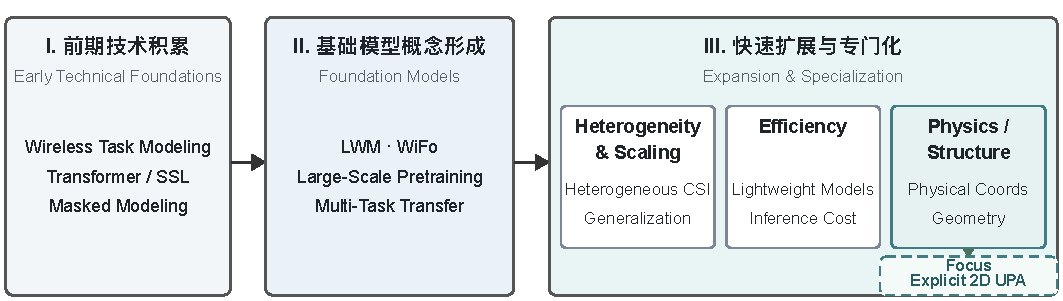
\includegraphics[width=\textwidth]{figures/fig1_wfm_timeline.pdf}
\caption{无线基础模型从前期技术积累、基础模型概念形成到异构化、规模化与物理结构感知方向快速扩展的发展脉络。本文关注其中二维 UPA 几何显式建模问题。}
\label{fig:timeline}
\end{figure*}

\subsection{信道与 CSI 基础模型的技术演进}

早期 CFM 的核心目标是形成统一的时空频信道表示。WiFo \cite{liu2025wifo} 将时空频 CSI 作为输入，用随机、时域和频域掩码重建学习信道结构，使同一模型可以服务多种配置下的信道预测。官方实现将天线作为一维轴处理，token patch 同时混合时间、频率和天线位置；这一结论来自官方源码审计，而不是仅依据论文叙述。

当任务范围扩展后，统一表示必须同时处理异构输入、任务差异和物理坐标。WiFo-2 \cite{liu2026wifo2} 面向异构无线系统设计并扩展任务范围；公开推理代码中的 \texttt{SinCos\_3D} 为时间、天线和频率三个 patch 轴分配表示子空间，但天线仍保持为一维展平轴。因此，其坐标体系是 \((time, antenna, frequency)\) 或 \((t,k,u)\)，尚未分解为 UPA 的行与列。这说明 WiFo 系列并非缺少物理坐标，而是采用了一维天线索引的坐标接口。

与 WiFo 不同，LWM \cite{alikhani2024lwm} 强调从大规模信道数据学习可迁移嵌入，并服务波束预测和用户定位等任务。围绕表示的可扩展性，HeterCSI \cite{jiang2026hetercsi} 用尺度自适应批构造和双掩码机制处理规模与场景异构，CSI-MAE \cite{jiang2026csimae} 研究跨场景与零样本迁移，ContraWiMAE \cite{guler2026contrawimae} 将掩码重建与掩码对比学习结合，CIR-CSI consistency 模型 \cite{jiang2025circsi,jiang2026csiclip} 则通过两种信道观测视图的一致性学习扩展表示。这些工作共同表明，CFM 的研究重点正在从单一输入格式的掩码重建转向异构数据下的可迁移表征。

表示能力最终需要转化为通信系统中的具体任务。WiFo-CF \cite{liu2026wifocf} 研究 CSI 反馈，WiFo-E \cite{wen2026wifoe} 研究端到端 FDD 预编码，WiFo-INR \cite{liu2026wifoinr} 用坐标条件化神经函数表示 CSI，WiCo-MG \cite{han2026wicomeg} 和 WiCo-PG \cite{sun2026wicopg} 将环境信息引入多径生成和路径损耗图生成。这些工作扩展了 CFM 的应用边界，但并不都直接面向二维阵列结构或部分阵列恢复。

规模与效率也随之成为不可回避的约束。Tiny-WiFo \cite{zhang2026tinywifo} 通过多组件自适应知识蒸馏获得约 5.5M 参数量级的模型，Scalable Pre-Trained Masked Channel Model \cite{guo2026scalable} 研究 5M 到 1B 参数的掩码信道补全，ComHymba \cite{yang2026comhymba} 和 WiMamba \cite{raviv2026wimamba} 探索状态空间模型或混合骨干以降低 token 复杂度。因此，本课题需要在相同协议下量化二维几何表示的边际贡献，并同时报告计算代价。

表~\ref{tab:cfm-tech} 对代表性 CFM 的输入、token、位置编码、掩码和阵列表示进行技术比较。表中“Unknown”表示尚未完成源码级或全文级确认，只表示证据状态，不构成否定性结论。

\begin{table*}[!t]
\caption{代表性 Channel/CSI Foundation Model 技术比较。模型结构字段仅填写已完成核验或论文明确说明的信息；Unknown 表示尚未确认。}
\label{tab:cfm-tech}
\centering
\scriptsize
\begin{tabular}{L{2.20cm}L{1.80cm}L{1.70cm}L{1.70cm}L{2.30cm}L{2.20cm}L{1.40cm}}
\toprule
Model & Input representation & Patch/token & Position encoding & Mask/pretraining & Scale/tasks & Array \\
\midrule
WiFo \cite{liu2025wifo} & \(T\times K\times U\); \(U\) flattened & \((4,4,4)\) & \((t,k,u)\) 3D SinCos & Random, temporal, frequency & 160K samples; prediction & Flattened \\
WiFo-2 \cite{liu2026wifo2} & \(T\times U\times K\); \(U\) flattened & 3D cuboid & \texttt{SinCos\_3D} & Random, temporal, frequency & 11.6B CSI points; 12 tasks & Flattened \\
Adaptive 3D-RoPE \cite{zhang2026adaptive3drope} & \(H\in\mathbb{C}^{T\times K\times U}\) & \((4,4,4)\) & Adaptive RoPE & Random, temporal, frequency & 144K train; reconstruction/prediction & Flattened \\
PilotWiMAE \cite{guler2026pilotwimae} & \((B,T,S,F)\), \(S=N_hN_v\) & \((1,4,4)\) & \((t,s,f)\) SinCos & Pilot-native masked reconstruction & 3.5/28 GHz; estimation/beam & Flattened \\
HeterCSI \cite{jiang2026hetercsi} & Heterogeneous CSI & Unknown & Unknown & Scale-aware batching, double masking & 12 datasets; reconstruction/prediction & Unknown \\
CSI-MAE \cite{jiang2026csimae} & CSI & Unknown & Unknown & Masked autoencoder & 3GPP datasets; cross-scenario & Unknown \\
ContraWiMAE \cite{guler2026contrawimae} & Wireless channel & Unknown & Unknown & Masked reconstruction + contrastive & Unknown; multi-task & Unknown \\
SPA-MAE \cite{chen2026spamae} & CSI with multipath prior & Unknown & Unknown & Physics-guided MAE & Unknown; reconstruction/estimation & Unknown \\
ComHymba \cite{yang2026comhymba} & CSI & 3D STF patch & Rotary PE & Domain-informed masking & Unknown; reconstruction, sensing, beam & Unknown \\
WALoMA \cite{makin2026waloma} & CSI & Unknown & Antenna-subcarrier PE & Adaptive low-rank MAE & Unknown; multi-task & Unknown \\
AirFM-DDA \cite{bian2026airfmdda} & Delay-Doppler-Angle & Unknown & Frame-structure-aware PE & Windowed attention & Unknown; prediction, estimation, beam & Unknown \\
WiFo-INR \cite{liu2026wifoinr} & Coordinate-conditioned function & Unknown & Coordinate-conditioned SIREN & Mixed masking & Unknown; reconstruction/feedback & Unknown \\
\bottomrule
\end{tabular}
\end{table*}

\subsection{从数据驱动表示到物理结构感知}

CFM 近期最明显的变化，是物理结构从训练数据中的隐式统计规律逐渐成为显式的模型接口。最基础的表现是时间、频率和天线轴的结构化。WiFo 的三类掩码将随机重建、时域预测和频域预测纳入统一预训练；WiFo-2 与 Adaptive 3D-RoPE 进一步把三轴坐标引入位置表示。Adaptive 3D-RoPE \cite{zhang2026adaptive3drope} 通过样本自适应的旋转频率尺度调制 \((t,k,u)\) 坐标，使相同坐标偏移在不同信道状态下产生不同的注意力交互。源码审计确认其实现了相对位移 \(\Delta t\)、\(\Delta k\) 和 \(\Delta u\)，但 \(\Delta u\) 位于一维展平天线 patch 轴，并不等价于行位移与列位移。

另一条线关注观测现实性。PilotWiMAE \cite{guler2026pilotwimae} 指出许多 CFM 假设完整 CSI 可直接获得，而实际系统往往只能观测含噪导频，因此其编码器直接接收导频观测，并将注意力分解为时间注意力和空间-频率联合注意力。源码审计确认物理发送阵列是 \(4\times 8\) UPA，但模型输入将 \((N_h,N_v)\) 展平为 \(S=N_hN_v\)，token patch 也包含 4 个展平天线元素。其空间建模因此发生在展平天线 patch 轴上，而不是二维阵列几何上。

物理结构也可以通过变换域和物理参数进入模型。AirFM-DDA \cite{bian2026airfmdda} 将 CSI 重参数化到时延-多普勒-角度域，用物理上更可分的轴描述多径结构；SPA-MAE \cite{chen2026spamae} 使用多径参数和稀疏变换域结构引导掩码自编码预训练。再加上坐标条件化和不变性研究，如 WiFo-INR \cite{liu2026wifoinr} 的坐标条件化函数以及 Physics Equivariance \cite{wang2026physicseq} 对物理等变性的讨论，可以看到几何与物理先验存在多种入口：坐标编码、变换域表示、注意力分解、导频观测或辅助监督。本课题选择的是阵列几何接口，即在 token 坐标和相对阵列位移中显式保留 UPA 结构。

\subsection{二维阵列表示与研究缺口}

在 MIMO/UPA 信道中，物理阵列天然具有行和列两个方向。假设第 \(r\) 行第 \(c\) 列阵元编号为
\begin{equation}
u=rN_v+c,\quad r=0,\ldots,N_h-1,\quad c=0,\ldots,N_v-1.
\label{eq:flatten}
\end{equation}
该映射是一一对应的，因此展平编号并不丢失阵元身份。问题的关键不在编号是否唯一，而在模型接口是否显式表达二维几何关系。当模型仅接收一维 \(u\)，且没有额外的阵列形状或行-列元数据时，同一行内的水平相邻、跨行垂直相邻、对角相邻以及二维距离相同的阵元在输入接口上并不具有不同的显式表示。以 \(4\times8\) 与 \(8\times4\) 两个 \(N=32\) 的 UPA 为例，相同的展平索引序列对应不同的物理几何。

这一判断关注模型接口，而不是断言展平模型在数学上无法学习几何。如果训练分布提供稳定的统计线索，模型可能从 CSI 数值中间接学习部分阵列关联；但仅由 \(u\) 构成的接口并没有显式给出 \(N_h\)、\(N_v\)、行相邻、列相邻或二维相对位移。因此，物理数据使用 UPA 并不等价于模型显式保留 UPA 拓扑。源码审计显示，PilotWiMAE 的数据生成配置使用 \(4\times8\) 平面阵列，但模型输入和 patch 坐标均为展平天线轴；Adaptive 3D-RoPE 的仿真数据可来自物理 UPA，但模型坐标仍是 \((t,k,u)\)；WiFo-2 的公开实现也保持一维天线轴。已有工作并非没有空间信息，而是在 token 接口处将二维阵列几何压缩为一维索引或在天线 patch 中混合多个阵元。

表~\ref{tab:upa-geometry} 进一步比较与 UPA geometry 高度相关的模型接口。表中的 No 仅用于源码审计已确认不存在对应结构的条目；对尚未完成同等审计的工作统一标记为 Unknown，不作为否定结论。

\begin{table*}[!t]
\caption{与二维 UPA geometry 高度相关模型的接口比较。No 表示源码级审计已确认；Unknown 表示尚未确认。}
\label{tab:upa-geometry}
\centering
\scriptsize
\begin{tabular}{L{2.40cm}L{1.80cm}L{1.15cm}L{2.10cm}L{1.90cm}L{2.15cm}L{3.00cm}}
\toprule
Model & Antenna representation & \(N_h,N_v\) & Token geometry & Relative geometry & Structured spatial mask & UPA shape generalization \\
\midrule
WiFo \cite{liu2025wifo} & \(U=N_hN_v\), flattened & \no & \((t,k,u)\) & None & No & Unknown \\
WiFo-2 \cite{liu2026wifo2} & \(U\), flattened & \no & \((t,u,k)\) & None & 1D antenna mask in source & Antenna count; shape Unknown \\
Adaptive 3D-RoPE \cite{zhang2026adaptive3drope} & \(U\), flattened & \no & \((t,k,u)\) & \(\Delta t,\Delta k,\Delta u\) & 1D antenna mask in code; main protocol unused & Unknown \\
PilotWiMAE \cite{guler2026pilotwimae} & \(S=N_hN_v\), flattened & \no & \((t,s,f)\) & None & No row, column, or block mask & Unknown \\
ComHymba \cite{yang2026comhymba} & Unknown & \unknown & 3D STF patch (claimed) & Unknown & Domain-informed masking & Unknown \\
WALoMA \cite{makin2026waloma} & Unknown & \unknown & Unknown & Unknown & Adaptive low-rank masking & Unknown \\
AirFM-DDA \cite{bian2026airfmdda} & Unknown & \unknown & Delay-Doppler-Angle axes & Unknown & Unknown & Claims antenna configurations \\
WiFo-INR \cite{liu2026wifoinr} & Unknown & \unknown & Coordinate function (claimed) & Unknown & Mixed masking & Claims CSI-size independence \\
\midrule
Proposed & Preserve \(N_h,N_v\) & \yes & \((t,k,r,c)\) & \(\Delta r,\Delta c\) & Antenna, row, column, block & Planned \(4\times8\) vs \(8\times4\) \\
\bottomrule
\end{tabular}
\end{table*}

图~\ref{fig:flatten-vs-upa} 给出了两种表示的概念差异。该图对比 \(H\in\mathbb{C}^{T\times K\times N}\) 的展平表示与 \(H\in\mathbb{C}^{T\times K\times N_h\times N_v}\) 的显式二维表示。

\begin{figure*}[!t]
\centering
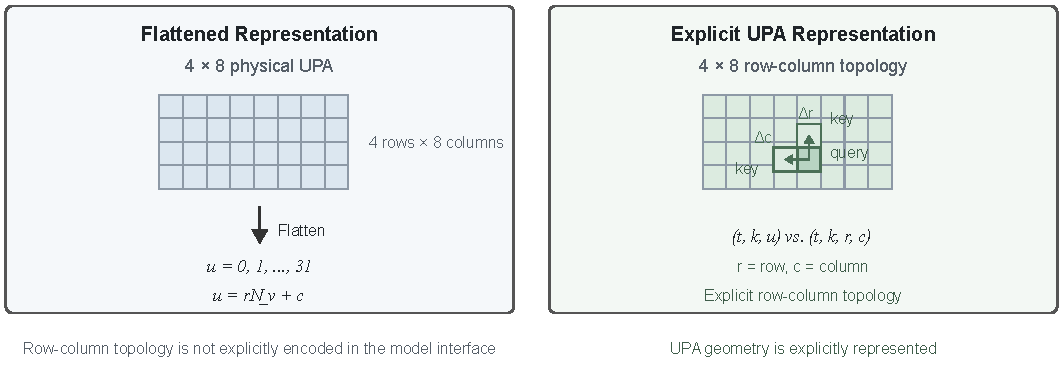
\includegraphics[width=\textwidth]{figures/fig2_flatten_vs_upa.pdf}
\caption{展平天线轴表示与显式二维 UPA 行-列拓扑表示的概念差异。}
\label{fig:flatten-vs-upa}
\end{figure*}

\subsection{现有研究不足}

上述综述说明，CFM 的研究缺口不在于缺少物理或空间先验，而在于不同物理结构进入模型接口的粒度并不相同。时间、频率、天线、时延、多普勒、角度和导频结构均已被显式利用；但在已审计的代表性工作中，二维平面阵列通常仍被压缩为一维天线轴，或在 patch embedding 阶段提前混合多个阵元。行-列拓扑、水平与垂直关系以及二维相对阵列几何尚未作为独立建模变量被系统检验。

这一缺口与现有方法的具体设计相互对应。Adaptive 3D-RoPE 覆盖了 \((t,k,u)\) 的三维相对旋转几何，PilotWiMAE 覆盖了导频原生输入和空间-频率注意力，WiFo-2 覆盖了时间、天线和频率的三维 token 坐标。源码审计尚未在这些工作中发现 \((t,k,r,c)\) token 坐标、分离的 \(\Delta r\) 与 \(\Delta c\) 相对几何，或 \(B_h(\Delta r,\Delta c)\) 形式的 UPA 注意力偏置。对于 ComHymba、WALoMA、AirFM-DDA、WiFo-INR 等尚未完成同等深度审计的工作，本报告保留 Unknown，不根据标题或摘要推测其阵列接口。

训练目标也需要与该接口问题对应。现有掩码任务主要集中于随机、时域、频域、导频或展平空间-频率重建，尚缺少针对二维阵列结构的行、列、局部二维块和部分阵列恢复的系统化验证。由此，本课题的核心问题可表述为：在 CFM 中显式保持并利用二维 UPA 行-列拓扑，能否带来可验证的表示与恢复收益。

\section{研究问题与研究目标}

\subsection{核心科学问题}

本课题的核心科学问题是：在信道基础模型中，显式保持二维 UPA 行-列拓扑，能否提高模型对无线信道空间结构的表示能力，并改善信道预测、重建及部分阵列恢复性能？

为使该问题可检验，本课题将其分解为四个相互衔接的层面。首先，在 token 化阶段，是否应避免过早融合多个阵元，使每根阵元先形成独立的局部时频表示，再由后续注意力学习阵元间关系。其次，对 UPA 而言，\((t,k,r,c)\) 是否比 \((t,k,u)\) 更适合描述 token 的物理位置，其中 \(r\) 为行索引，\(c\) 为列索引。再次，显式建模 \(\Delta r\) 与 \(\Delta c\)，并用可分离注意力偏置表示二维位移，是否比仅依赖展平 \(\Delta u\) 或绝对位置编码带来额外收益。最后，行、列和二维块等结构化空间掩码是否能够增强模型对空间相关结构和部分阵列恢复任务的学习能力。

\subsection{研究目标}

本课题的总体目标是构建并验证一个面向二维 UPA 的几何感知信道基础模型。具体目标包括：
\begin{enumerate}
\item 建立阵元独立的时频 patch embedding，使阵元间关系不在嵌入阶段被提前混合；
\item 构造 \((t,k,r,c)\) 四维 token coordinate，将 UPA 行和列作为显式模型轴；
\item 设计可分离的二维 UPA 相对几何，使注意力区分水平距离、垂直距离和二维方向关系；
\item 设计阵元、行、列和二维块结构化掩码，与随机、时域和频域任务形成统一掩码重建预训练；
\item 通过受控消融、跨场景实验和 UPA 形状泛化验证各组件的独立与联合贡献。
\end{enumerate}

\section{拟采用的研究方法}

\subsection{总体架构与研究路径}

设训练样本为
\begin{equation}
\mathbf{H}\in\mathbb{C}^{B\times T\times K\times N_h\times N_v},
\end{equation}
其中 \(B\) 为批大小，\(T\) 为时间符号数，\(K\) 为子载波或频点数，\(N_h\) 为 UPA 行数，\(N_v\) 为 UPA 列数。与研究问题对应，模型由四个层次构成：阵元独立时频表示、显式二维 UPA 坐标、二维相对几何注意力以及结构化空间掩码预训练。整体流程为
\[
\begin{aligned}
&\mathrm{CSI}\rightarrow \text{阵元独立时频表示}\\
&\rightarrow \text{显式 UPA 坐标}\rightarrow \text{几何感知 Transformer}\\
&\rightarrow \text{掩码重建与信道预测}.
\end{aligned}
\]

图~\ref{fig:framework} 给出本课题的总体方法框架。

\begin{figure*}[!t]
    \centering
    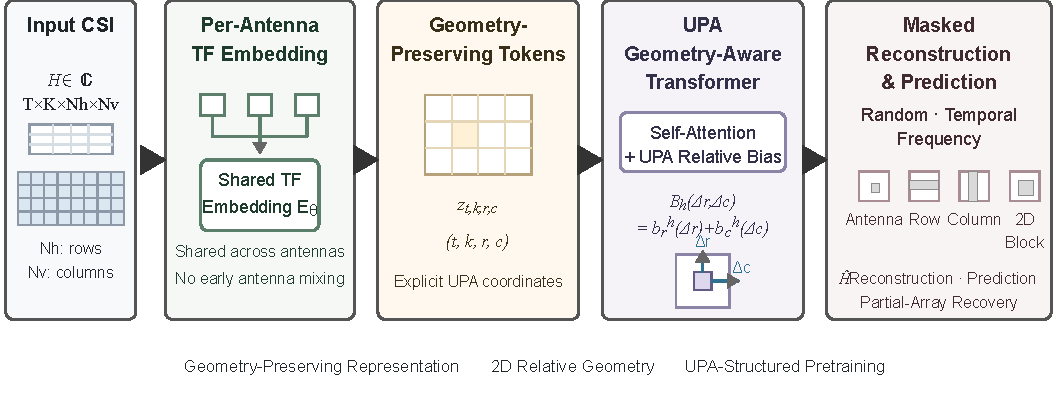
\includegraphics[width=\textwidth]{figures/fig3_upa_framework.pdf}
    \caption{面向二维均匀平面阵列的几何感知信道基础模型总体框架。模型首先以共享的阵元独立时频嵌入提取局部特征，并保留 $(t,k,r,c)$ 四维 token 坐标；随后通过基于 $(\Delta r,\Delta c)$ 的二维相对几何偏置建模阵元关系，并结合随机、时域、频域以及阵元、行、列和二维块结构化掩码进行统一自监督重建。}
    \label{fig:framework}
\end{figure*}

\subsection{阵元独立时频表示}

阵元独立表示的作用是将天线间关系的建模从特征提取阶段推迟到注意力阶段。对每个阵元 \((r,c)\)，模型共享同一时频 patch embedding 参数，提取局部时频特征。若时间 patch 长度为 \(p_t\)，频率 patch 长度为 \(p_k\)，可写为
\begin{equation}
\begin{aligned}
\mathbf{z}_{t,k,r,c}
=E_\theta\big(&
[\Re\mathbf{H}_{t:t+p_t-1,k:k+p_k-1,r,c},\\
&\Im\mathbf{H}_{t:t+p_t-1,k:k+p_k-1,r,c}]
\big),
\end{aligned}
\end{equation}
其中 \(E_\theta\) 对所有 \((r,c)\) 共享。这样，每枚 token 对应一个阵元的局部时频 patch，而不是多个阵元的混合特征；阵元间关系随后由几何感知注意力显式学习。该设计的关键不是使用何种具体卷积算子，而是保持阵元级 token 结构，使行、列坐标和空间掩码能够作用在同一建模粒度上。

这一选择会带来明确的计算代价。以 \(p_t=p_k=4\) 为例，若 WiFo-like 模型将 4 根天线混合进一个 token，则阵元级表示的 token 数约为其 4 倍，全局注意力的理论开销约按 token 数平方增长。因此，后续实验将同时报告参数量、显存、FLOPs 和推理时间，以评价性能与效率的权衡。

\subsection{显式二维 UPA 坐标}

每枚 token 被赋予四维坐标
\begin{equation}
\mathbf{x}=(t,k,r,c),
\end{equation}
分别对应时间 patch、频率 patch、UPA 行索引和列索引。与 \((t,k,u)\) 相比，该表示不再依赖式~\eqref{eq:flatten} 中的一维展平索引。这里的关键是接口显式性：\(u=rN_v+c\) 可以唯一编号阵元，但当模型只接收展平索引且没有阵列形状或行-列元数据时，输入接口本身不显式编码 \(4\times8\) 与 \(8\times4\) 的二维拓扑差异。\((t,k,r,c)\) 则将行和列作为模型变量保留下来。

\subsection{二维相对几何与注意力偏置}

为使注意力直接感知二维阵列位移，在每个注意力头中引入可分离相对偏置。设第 \(h\) 个头的行偏置表为 \(b_r^h(\Delta r)\)，列偏置表为 \(b_c^h(\Delta c)\)，则
\begin{equation}
B_h(\Delta r,\Delta c)
=b_r^h(\Delta r)+b_c^h(\Delta c).
\label{eq:bias}
\end{equation}
对于查询 token \((r_i,c_i)\) 和键 token \((r_j,c_j)\)，\(\Delta r=r_i-r_j\)，\(\Delta c=c_i-c_j\)。注意力分数可写为
\begin{equation}
A_{ij}^{(h)}
=\frac{\mathbf{q}_i^{(h)\top}\mathbf{k}_j^{(h)}}{\sqrt{d_h}}
+B_h(r_i-r_j,c_i-c_j).
\end{equation}

该偏置使模型能够显式区分水平邻近、垂直邻近、对角关系以及不同二维距离。采用可分离形式而不是完整的 \((\Delta r,\Delta c)\) 偏置表，一方面控制参数和内存，另一方面便于分别消融行方向与列方向偏置。图~\ref{fig:relative-geometry} 给出相对几何示意。

\begin{figure*}[!t]
\centering
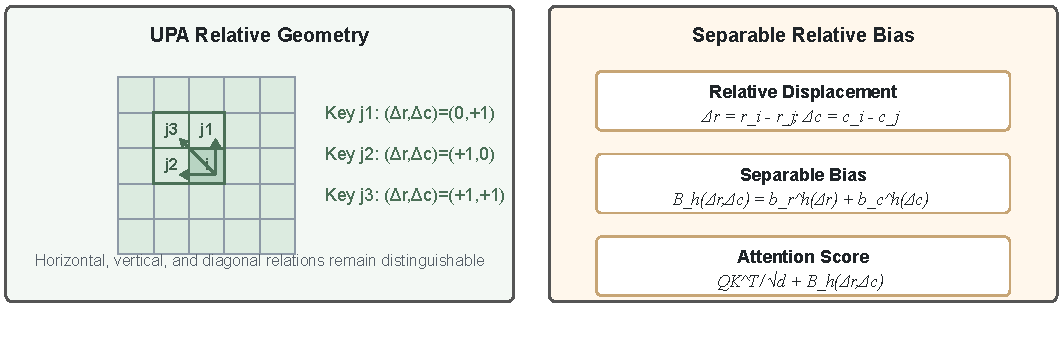
\includegraphics[width=\textwidth]{figures/fig4_relative_geometry.pdf}
\caption{二维 UPA 行、列相对位移及可分离相对注意力偏置示意。}
\label{fig:relative-geometry}
\end{figure*}

\subsection{UPA 结构化空间掩码}

在随机、时域和频域掩码之外，本课题引入四类空间掩码：阵元掩码随机遮蔽若干完整阵元，行掩码遮蔽一行或多行阵元，列掩码遮蔽一列或多列阵元，二维块掩码遮蔽局部矩形区域并形成部分阵列恢复任务。这些掩码与已有任务共同构成统一的掩码重建预训练。其目的不是增加掩码类型本身，而是使预训练目标显式覆盖 UPA 的结构化缺失模式：行掩码考察行间相关性的利用，列掩码考察列间相关性的利用，二维块掩码则对应局部阵列缺失下的空间重建能力。图~\ref{fig:masks} 给出四类掩码示意。

\begin{figure*}[!t]
\centering
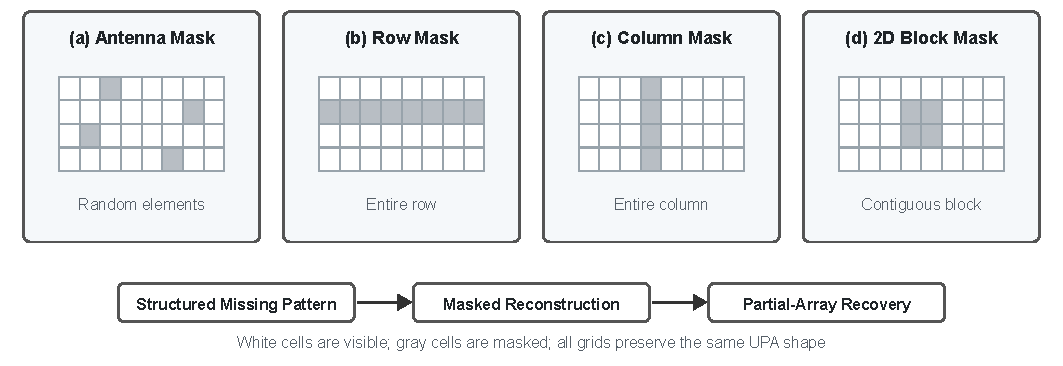
\includegraphics[width=\textwidth]{figures/fig5_structured_masks.pdf}
\caption{面向二维 UPA 拓扑的阵元、行、列和二维块结构化空间掩码策略。}
\label{fig:masks}
\end{figure*}

\section{拟创新点}

\subsection{几何保持型信道表示方法}

本课题拟在 token 化过程中保持阵元级表示，将单一天线索引分解为行和列，并构造 \((t,k,r,c)\) 联合坐标。与物理数据使用 UPA 但模型输入仍为 \(N=N_hN_v\) 的做法相比，该方法使二维阵列结构直接参与模型接口，而不是只存在于数据生成参数中。

\subsection{二维相对位移感知的几何注意力机制}

本课题拟设计式~\eqref{eq:bias} 所示的可分离 UPA 相对几何偏置，使注意力显式感知 \(\Delta r\) 和 \(\Delta c\)。该机制区别于一维相对天线索引，也区别于绝对位置编码，其目标是以较少参数表达二维阵列中的方向和距离关系。

\subsection{面向二维阵列拓扑的结构化自监督预训练}

本课题拟利用阵元、行、列和二维块掩码构造结构化空间重建任务，研究模型对部分阵列恢复和空间相关结构的学习能力。相比随机、时域和频域掩码，该目标直接对应二维阵列的结构化缺失与部分恢复场景。

Conv2d、Transformer、四维正弦余弦编码或掩码自编码器本身不单独构成创新点。本课题的创新集中于这些组件如何共同服务二维 UPA 几何保持、相对几何建模和结构化空间预训练。

\section{实验设计}

\subsection{总体消融设计}

实验的首要任务是隔离表示、坐标、几何偏置和预训练目标的贡献。为此，实验将以 WiFo-like 展平天线表示作为基础基线，并构造递进式消融：A 加入阵元独立表示；B 在 A 的基础上加入显式二维 UPA 坐标；C 在 B 的基础上加入二维相对几何；D 在 C 的基础上加入空间预训练；Full 使用完整结构化空间掩码与完整模型。该设计使每一层差异都对应一个明确的技术假设。

所有消融将保持相同数据划分、优化器、学习率调度、掩码比例、输入噪声协议、评估指标和随机种子策略。后续正式实验计划至少使用三个随机种子，并报告均值、标准差或置信区间。

\subsection{任务与指标}

评测任务覆盖时域预测、频域预测、随机重建和空间重建；空间重建进一步包括阵元、行、列和二维块模式。主要指标为被遮蔽位置上的 NMSE，并同时报告参数量、显存占用和单样本推理时间；必要时补充 FLOPs 与训练时间，以评价几何感知带来的计算代价。所有 NMSE 将使用相同的目标区间和归一化方式。

\subsection{基线与外部比较}

内部基线以 WiFo-like 展平模型为主，用于隔离阵列表示差异本身。外部比较将优先选择与研究问题相邻的方法：官方 WiFo-Small/Base 权重用于检验相同任务与相同掩码比例下的表现；Tiny-WiFo 的参数规模与本课题相近；HeterCSI 直接研究异构 CSI 预训练；Adaptive 3D-RoPE 直接研究物理坐标旋转编码；PilotWiMAE 关注导频原生输入和空间-频率注意力。在计算条件允许时，还将评估 WiFo-2 或 ComHymba 等更强或更高效模型。不同训练规模、数据集、掩码比例和输入噪声协议的结果不会放入同一数值比较表，外部公开结果只作为研究上下文。

\subsection{泛化实验}

泛化实验包括三个层次：场景泛化在不同场景、速度、LoS/NLoS 和信道生成配置上评估零样本或少样本性能；阵列规模泛化在不同 \(N_h,N_v\) 上检验相对偏置的覆盖范围和外推能力；UPA 形状泛化则在相同 \(N=32\) 下比较 \(4\times8\) 与 \(8\times4\)。其中形状泛化最能直接检验研究问题：当模型仅接收展平索引且没有阵列形状或行-列元数据时，接口本身不区分两种二维拓扑；若显式行-列表示有效，则应在相同阵元数量下表现出更稳定的形状适应能力。

\section{初步实验}

\subsection{实验设置}

初步实验采用 D4 数据集，配置为 \(T=16\)、\(K=32\)、\(4\times8\) UPA、UMa+LoS、30--100 km/h。数据划分为训练 9000、验证 2000、测试 1000。训练 20 个 epoch，批大小为 16，使用 AMP 混合精度，随机种子为 17。WiFo-like 与 Full 的参数量分别为 5.40M 和 5.36M，容量基本相当。该实验定位为开题前的方向性验证，而不是完整论文实验。

训练任务为随机、时域、频域和空间任务混合采样。随机掩码比例为 0.85，时域和频域掩码比例均为 0.50。空间任务由阵元、行、列和二维块掩码组成，其中阵元策略目标掩码比例为 0.25，行、列和块掩码按合法规模采样并保持空间可见率不低于 0.5。

\subsection{结果与分析}

表~\ref{tab:preliminary} 给出测试集结果。在参数量差异约 0.9\% 的受控设置下，Full 在时域、频域和随机重建三个共同任务上均低于 WiFo-like，并新增了空间重建任务的可评估接口。该结果初步说明显式 UPA 建模具有继续研究价值，但仍需要系统消融和多种子实验确定贡献来源。

\begin{table}[!htbp]
\caption{D4 初步实验结果。表中为 masked positions 上的测试 NMSE；WiFo-like 不支持空间掩码任务。}
\label{tab:preliminary}
\centering
\begin{tabular}{lccc}
\toprule
Task & WiFo-like & Full & Improvement \\
\midrule
Temporal & 0.1091 & 0.0525 & 0.0566 \\
Frequency & 0.2336 & 0.1986 & 0.0350 \\
Random & 0.2303 & 0.1859 & 0.0444 \\
Spatial & --- & 0.3445 & --- \\
\midrule
Parameters & 5.40M & 5.36M & --- \\
\bottomrule
\end{tabular}
\end{table}

该实验的边界也很清楚。它只使用单一数据集、20 个 epoch 和单一随机种子，尚未覆盖更大规模预训练；WiFo-like 是内部公平消融基线，不是官方 WiFo 或最新 CFM 的完整复现；空间重建 NMSE 是新增任务，不能与不支持该任务的模型直接比较；同时，Full 的 token 数显著高于 WiFo-like，训练时间约增加 18 倍。因此，本节结果只用于支持“该方向值得继续验证”，后续仍需通过系统消融、多种子训练和跨场景实验建立更可靠的结论。

\section{研究计划}

本课题拟按以下阶段推进。
\begin{enumerate}
\item \textbf{文献调研与审计深化：} 完成表~\ref{tab:cfm-tech} 中 Unknown 字段的全文和源码核验，重点补齐 ComHymba、WALoMA、AirFM-DDA、WiFo-INR 和 prompt-guided multi-band CSI FM 的阵列表示；
\item \textbf{模型完善：} 固化张量接口、位置编码、相对偏置和结构化掩码，补齐单元测试与复现实验；
\item \textbf{消融实验：} 完成 WiFo-like、A、B、C、D 和 Full 的多种子训练，统计各组件贡献；
\item \textbf{多场景验证：} 在不同场景、速度和信道配置下评估零样本与少样本泛化；
\item \textbf{UPA 形状泛化：} 重点比较 \(4\times8\) 与 \(8\times4\)，并扩展到其他阵列规模；
\item \textbf{复杂度分析：} 系统报告参数量、显存、FLOPs、训练时间和推理延迟，评估性能-效率权衡；
\item \textbf{结果分析与论文撰写：} 结合 CFM-Bench 或统一评测协议解释结果边界，完成学位论文和投稿版本。
\end{enumerate}

\section{风险与应对}

本课题的主要风险来自三个方面。首先是计算复杂度：阵元级表示会增加 token 数，全局注意力复杂度按平方增长，后续将在复杂度分析中评估性能与效率的权衡。其次是归因风险：性能增益可能来自容量、训练任务或掩码难度差异，而不是二维几何本身；应对策略是严格控制参数量、数据划分、优化器、掩码比例和随机种子，并通过 A/B/C/D 分层消融定位贡献来源。最后是相关工作更新速度：Adaptive 3D-RoPE、PilotWiMAE、HeterCSI 和 WiFo-2 已覆盖物理坐标、导频原生输入、异构预训练和三维 token 坐标，本课题将保持研究定位在 UPA 行-列几何，并持续更新文献与源码审计状态。

\section{结语}

本课题从 WFM 与 CFM 的发展出发，梳理了研究关注点从任务迁移、异构表示向物理结构接口演进的过程，并进一步聚焦二维 UPA 的行-列拓扑是否应在 CFM 中显式保留。拟通过阵元独立时频表示、\((t,k,r,c)\) 坐标、可分离二维相对几何和结构化空间掩码验证该问题。初步 D4 受控实验提供了继续研究的信号，但完整结论仍需系统消融、多种子训练、跨场景验证和多几何形状实验支持。

\section*{文献核验说明}

本报告中的正式出版信息、arXiv 标识和 DOI 于 2026-09-28 通过出版社/Crossref/arXiv 元数据核验。Adaptive 3D-RoPE、PilotWiMAE、WiFo 和 WiFo-2 的结构结论进一步参考了官方源码审计，对应审计 commit 的短标识分别为 \texttt{f0df7e6}、\texttt{0829fc2}、\texttt{a0889e1} 和 \texttt{f9a9368}；完整 commit 哈希和逐项证据保留在本项目的源码审计记录中。未完成源码级审计的条目在表中标记为 Unknown，后续不得将其改写为 Yes 或 No。

\IEEEtriggeratref{31}
\bibliographystyle{IEEEtran}
\bibliography{references}

\end{document}
